\chapter{Additional Experimental Results}
\label{app:results}

\TODO{for all tables that basically just restate in numbers some figure / chart already present in the main text, say that in their caption or introductory paragraphs i.e. "The values in this table correspond directly to those shown in Figure X in the main text." or somoething simialr}

\TODO{try to write sentences that don't feature the ';' as a way to seprarate stencens i prefer sentences that are shorter but clearer}

\TODO{overall, recheck that the different parts of the appendix are correctly linked back in the main text by checking the label/refs usage etc. check that the references are correctly pointing to the intended sections, figures, and tables in the main text.}

\TODO{the aim for this appendix should be to be a comprehensive repository of supplementary material that supports the main experimental results, providing additional numeric tables, extended figures, and detailed validation data. that means that anythign that isn't directly supporting the main experimental results should be excluded and removed. even if the reuslt seem interesting like 6/10 it should be removed. i only want the appendix to contain extra material like data that I couldn't fit in the main text, not be an extra chapter fitted in the appendix because I didn't have room in the 30 pages. remove anything thats not useful or not major}

\TOFIX{reread once finished}{This appendix collects material that supports Chapter~\ref{chap:experiments}, including extended numeric tables behind figures shown in the main text, supplementary figures for the search algorithms of Chapter~\ref{chap:algorithms}, and one additional optimality-scope result. Sections are grouped by what they support rather than one per table, and every table or figure below is referenced from the main-chapter passage that motivates it.}

\section{Experimental Parameters}
\label{app:params}

\TOFIX{maybe remove?}{Table~\ref{tab:params} summarizes every parameter varied anywhere in Chapter~\ref{chap:experiments}, alongside the reference value used whenever it is held fixed, and the section in which it is swept.}

\begin{table}[ht]
    \centering
    \small
    \begin{tabular}{p{5cm}lllp{3cm}}
        \toprule
        Parameter & Symbol & Reference ($\mathcal{N}_{\mathrm{ref}}$) & Swept ranges & Where varied \\
        \midrule
        Hop count & $N$ & 10 & 10--28 & Section~\ref{sec:exp:budget} \\
        Hop length & $\ell_i$ & 2~km & \{1, 2, 3, 4\}~km & Section~\ref{sec:exp:heterogeneous} \\
        Tree-encoding branching vector & $\vec b^{(i)}$ & $(16,14,1)$ & -- & not varied \\
        BSM arm count & $k_i$ & 18 & 6, 18 & Section~\ref{sec:exp:netgen} \\
        Inner-qubit error rates & $\{p_X^{\mathrm{in}},p_Z^{\mathrm{in}}\}_i$ & 0 & [0, $3\!\times\!10^{-3}$] & Section~\ref{sec:exp:netgen} \\
        Photon survival probability & $\eta_i$ & 0.912 & $10^{-0.2 \ell_i/10}$ & Section~\ref{sec:exp:heterogeneous} \\
        Outer-photon depolarizing rate & $e_d$ & 0.01 & $[0,\,0.01]$ & Section~\ref{sec:exp:edsweep} \\
        Memory dephasing rate & $\gamma$ & 0 & $[0,\,10^5]$ & Section~\ref{sec:exp:timing} \\
        Propagation speed & $c$ & $2\!\times\!10^5$~km/s & -- & not varied \\
        Emission delay & $\tau_{\mathrm{emit}}$ & 0 & $[10^{-4},\,1]$ & Section~\ref{sec:exp:timing} \\
        Generation-cost budget & $E_{\max}$ & 100 & 50--280 & Sections~\ref{sec:exp:headline}--\ref{sec:exp:budget} \\
        \bottomrule
    \end{tabular}

    \caption{Experimental parameters. The reference column gives the nominal value used unless a parameter is varied in the indicated experiment. All parameters not listed as varying follow the Integrating paper's~\cite{Benchasattabuse2025Integrating} reference configuration $\mathcal{N}_{\mathrm{ref}}$ (Section~\ref{sec:model:network}). The tree branching factor is not varied because it does not affect the objectives $F$, $C$, or $R$ introduced in Chapter~\ref{chap:model}. Uniform hop-length scaling likewise leaves relative schedule comparisons unchanged; heterogeneous hop lengths are considered separately in Section~\ref{sec:exp:heterogeneous}.}
    \label{tab:params}
\end{table}

\section{Extended Physics Validation}
\label{app:validation}

Section~\ref{sec:exp:validation} reports the evaluator's agreement with the Integrating paper's Fig.\,5~\cite{Benchasattabuse2025Integrating}, \TOFIX{rephrase}{similarly at $e_d=0.01$}. Table~\ref{tab:app:validation} and Figure~\ref{fig:app:validation} give the evaluator's fidelity output for the raw, heralded-pumping, and optimistic-pumping canonical schedules (Section~\ref{sec:bg:decoherence}) across the full $e_d \in [0, 0.01]$ used throughout Chapter~\ref{chap:experiments}.

\TOFIX{the source paper's fig 5 is exactly reproduced in fig:app:validation so idk why this paragraph seems to say there is only 2 published points...? make sure this paragraph phrases correctly that my evaluator reproduces exactly the values of the paper; verify previous paragraph and the conten of chapter 6 as well}{The source paper publishes numeric reference values at only two points on this grid, $e_d=0.000$ and $e_d=0.010$: approximately $\{1.000, 1.000, 1.000\}$ and $\{0.823, 0.917, 0.929\}$ respectively, for the same three schedules in the same order. The evaluator matches both to at least three significant figures, and to four at $e_d=0.010$ (the values already quoted in Section~\ref{sec:exp:validation}). \TOFIX{maybe rephrase?}{The other nine intermediate rows have no corresponding published value to compare against, since the source paper's own Fig.\,5 does not report numeric values between its two published points but are still featured here for completeness}.}

\TODO{highlight in bold the evaluator's output that matches the source paper's published values.}

\begin{table}[h]
    \centering\small
    \begin{tabular}{cccc}
        \hline
        $e_d$ & $F_{\text{raw}}$ & $F_{\text{baseline (heralded)}}$ & $F_{\text{flexible (optimistic)}}$ \\
        \hline
        0.000 & \textbf{1.0000} & \textbf{1.0000} & \textbf{1.0000} \\
        0.001 & 0.9803 & 0.9932 & 0.9933 \\
        0.002 & 0.9610 & 0.9861 & 0.9866 \\
        0.003 & 0.9422 & 0.9787 & 0.9799 \\
        0.004 & 0.9239 & 0.9710 & 0.9730 \\
        0.005 & 0.9061 & 0.9629 & 0.9661 \\
        0.006 & 0.8887 & 0.9544 & 0.9591 \\
        0.007 & 0.8717 & 0.9456 & 0.9519 \\
        0.008 & 0.8552 & 0.9364 & 0.9446 \\
        0.009 & 0.8391 & 0.9268 & 0.9372 \\
        0.010 & \textbf{0.8234} & \textbf{0.9168} & \textbf{0.9295} \\
        \hline
    \end{tabular}

    \caption{Evaluator-derived fidelity vs.\ $e_d$ for the three canonical schedules of Section~\ref{sec:bg:decoherence}, at $N=10$. Bold rows ($e_d=0.000$ and $e_d=0.010$) are the only two points with a published reference value to compare against (see text).}
    \label{tab:app:validation}
\end{table}

\begin{figure}[ht]
    \centering
    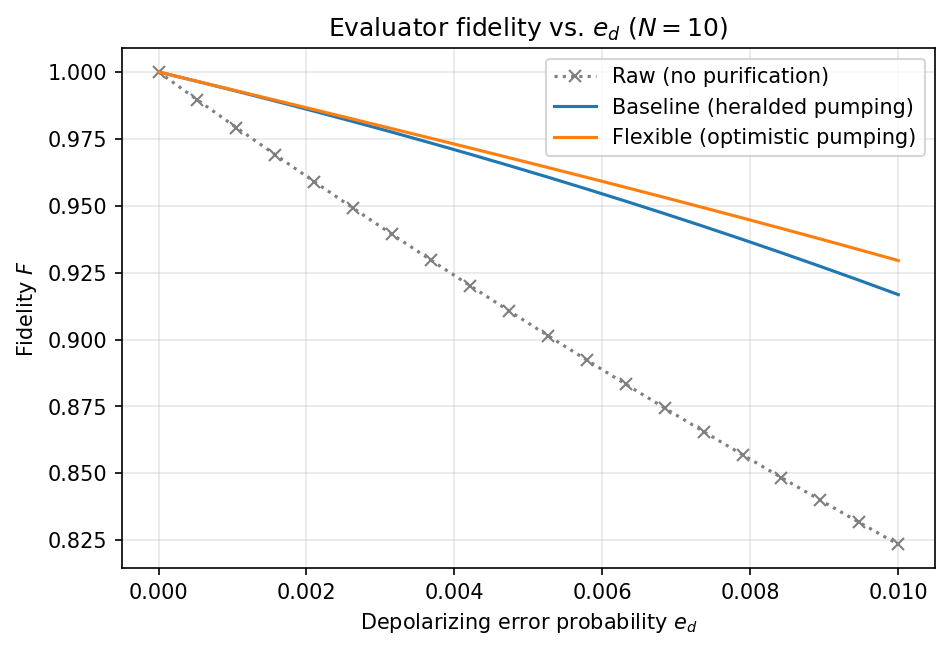
\includegraphics[width=0.7\textwidth]{figures/appendix/fidelity_vs_ed_validation.png}
    \caption{\TOFIX{add that this figure reproduces the source paper's Fig.\,5 exactly}{Evaluator fidelity vs.\ $e_d$ for the three canonical schedules of Table~\ref{tab:app:validation}, $N=10$. The raw chain degrades fastest; both pumping variants track closely, with the optimistic variant consistently slightly ahead of the heralded one over the whole range (Section~\ref{sec:disc:optimistic}).}}
    \label{fig:app:validation}
\end{figure}
\FloatBarrier

\section{Extended Network and Heterogeneity Comparisons}
\label{app:networks}

This section gives the full numeric backing for the two network-generalization experiments of Section~\ref{sec:exp:comparison}: uniformly applied non-ideal parameters (Section~\ref{sec:exp:netgen}) and per-hop heterogeneous networks (Section~\ref{sec:exp:heterogeneous}).

\subsection{Network Generalization Full Comparison}
\label{app:netgen}

Section~\ref{sec:exp:netgen} summarizes the network-generalization result. Table~\ref{tab:netgen} gives the full numeric comparison (cost, fidelity, and rate) behind Figure~\ref{fig:netgen}, across both tested \Gls{bsm} arm counts.

\begin{table}[h]
\centering
\caption{Optimizer versus the paper schedule under two non-ideal network configurations. Both use $N=10$, $e_d=0.01$, $E_{\max}=100$, $\gamma=0$, and non-zero inner-qubit error $p_X^{\mathrm{in}}=p_Z^{\mathrm{in}}=3\times10^{-3}$, unlike the source paper's idealized inner-qubit assumption. The configurations differ in the number of redundant \Gls{bsm} arms per hop. A schedule is feasible when $F\ge F_{\min}=0.9$.}
\label{tab:netgen}
\small
\begin{tabular}{llcccc}
\hline
Config & Schedule & $C$ & $F$ & Rate & Feasible \\
\hline
18 arms & Paper schedule & 100 & 0.67 & 103.18 & \textbf{no} \\
18 arms & Matched-cost & 100 & 0.90 & 25.31 & yes \\
18 arms & Budget-relaxed & 80 & 0.90 & 85.30 & yes \\
\hline
6 arms & Paper schedule & 100 & 0.87 & 871.55 & \textbf{no} \\
6 arms & Matched-cost & 100 & 0.93 & 681.56 & yes \\
6 arms & Budget-relaxed & 60 & 0.91 & 2096.91 & yes \\
\hline
\end{tabular}
\end{table}

\subsection{Heterogeneous Weak-Link Contrast}
\label{app:weaklink}

Section~\ref{sec:exp:heterogeneous} summarizes both the designed five-hop weak-link case and the 100-network random sample. Table~\ref{tab:weaklink} gives the full numeric comparison for the designed case: one hop with a $12\times$ higher inner-qubit error rate than its neighbours.

% Figure~\ref{fig:app:weaklink-allocation} shows how the two schedules allocate resources across that chain.

\begin{table}[ht]
    \centering
    \small
    \begin{tabular}{lcccc}
        \hline
        Schedule & $C$ & $F$ & Rate & Feasible \\
        \hline
        Best uniform link-level recipe & 40 & 0.88 & 1738.32 & \textbf{no} \\
        Optimizer's schedule & 38 & 0.90 & 1798.57 & yes \\
        \hline
    \end{tabular}

    \caption{Designed weak-link contrast for a heterogeneous $N=5$ network at $e_d=0.01$, $E_{\max}=50$, and $F_{\min}=0.9$. One hop has an inner-qubit error rate $12\times$ higher than its neighbours. The uniform link-level baseline uses the same purification configuration at every hop, whereas the optimizer may allocate resources differently across hops. A schedule is feasible when $F\ge F_{\min}$.}
    \label{tab:weaklink}
\end{table}

% \TODO{regenerate figure so that legend is both bigger font and without a border, below the figure}

% \begin{figure}[ht]
%     \centering
%     
\includegraphics[width=0.75\textwidth]{figures/results/weak_link_allocation.png}
%     \caption{Per-hop \texttt{GenNode} allocation for the optimizer's schedule and the best uniform link-level recipe, against the per-hop inner-qubit error rate, for the weak-link network of Table~\ref{tab:weaklink}. The optimizer spends less at hop 3 and reallocates the saved cost to the noisier hop 2, while the uniform recipe cannot vary its allocation across hops by construction.}
%     \label{fig:app:weaklink-allocation}
% \end{figure}
% \FloatBarrier

\TOFIX{rephrase, sounds too AI}{Figure~\ref{fig:app:heterogeneity} extends this single designed case to the full 100-network random sample}. It plots the optimizer's rate improvement over the best feasible uniform recipe, against each network's per-hop noise heterogeneity \TOFIX{what does this mean?}{(coefficient of variation of inner-qubit error rate across hops)}. Improvement is concentrated at \TOFIX{again too AI + what does it mean}{low-to-moderate heterogeneity}, where a single noisier hop still leaves room for the optimizer to reallocate resources profitably; the points sitting on the zero line are the ties noted in Section~\ref{sec:exp:heterogeneous}, \TOFIX{good but don't phrase with a not X but Y pattern like AI}{not cases where the optimizer underperforms}.


\TODO{regen figure, make legend's font bigger; rephrase the legends content maybe also color some points that are "performing" better? maybe not idk}

\begin{figure}[ht]
    \centering
    
\includegraphics[width=0.75\textwidth]{figures/results/random_sweep_improvement_vs_heterogeneity.png}
    \caption{Optimizer rate improvement over the best feasible uniform link-level recipe vs.\ per-hop noise heterogeneity, across the 100 random $N=6$ networks of Section~\ref{sec:exp:heterogeneous}. Points on the zero line are ties, not losses (Section~\ref{sec:disc:synthesis}).}
    \label{fig:app:heterogeneity}
\end{figure}
\FloatBarrier

\section{Extended Cost-Quality and Optimality Results}
\label{app:costquality}

\subsection{Alternative Objectives, Full Comparison}
\label{app:objectives}

Section~\ref{sec:exp:objectives} summarizes the objective-substitution result; Table~\ref{tab:app:objectives} gives the full five-objective comparison it draws from, at $N=10$ and $e_d=0.01$.

\begin{table}[ht]
    \centering
    \small
    \begin{tabular}{lccc}
        \hline
        Objective & $C$ & $F$ & Rate \\
        \hline
        Maximize rate & 60 & 0.9063 & 6195.95 \\
        Maximize fidelity, paper-rate floor & 80 & 0.9351 & 4804.58 \\
        Maximize fidelity, matched-rate floor & 80 & 0.9351 & 4804.58 \\
        Minimize cost, $F \ge 0.9$ only & 60 & --- & 1239.19 \\
        Minimize cost, $F \ge 0.9$ and $R \ge 4804.58$ & 60 & --- & 6195.95 \\
        \hline
    \end{tabular}

    \caption{Objective-substitution comparison at $N=10$, $e_d=0.01$: five objective definitions with no change to the search algorithm.}
    \label{tab:app:objectives}
\end{table}

\section{Search Algorithm Diagnostics}
\label{app:searchalgos}

\TODO{goal of this section is to justify the chosen beam width value and that beam search scales comparably to the exact dynamic program once same-span pumping is enabled. focus on that}

\TOFIX{which? does it mean instead "the following observations/diagnostics"}{These diagnostics} justify two implementation choices used throughout Chapter~\ref{chap:experiments}: the default beam width $w_{\mathrm{beam}}=25$ (Section~\ref{sec:alg:beam}) and the claim that beam search scales comparably to the exact dynamic program once same-span pumping is enabled (Section~\ref{sec:alg:pumping}).

\TOFIX{unclear and confused}{Figure~\ref{fig:app:beamwidth} shows why $w_\text{beam}=25$ was chosen as the default beam width: at $N=10$, wall-clock search time grows mildly up to a beam width of about 16 and then sharply beyond it, while the best rate found is already flat across the entire tested range, so widening the beam past 25 buys no further quality improvement at this configuration. Separately, at $N=6$, where the exact dynamic program (Section~\ref{sec:alg:dp}) remains tractable, beam search matches its exact optimum at every beam width tested from 1 to 32, with zero gap throughout -- confirming that this determinism holds even at the smallest beam widths, not only at the default.}

\TODO{regenerate figure to fix position and size of legend (to be bigger and not positioned middle left but top left in a box with larger font.) the blue line is also literally just a straight line on the graph so it looks weird. overall that graph is unreadable with 3 different axes.}

\begin{figure}[ht]
    \centering
    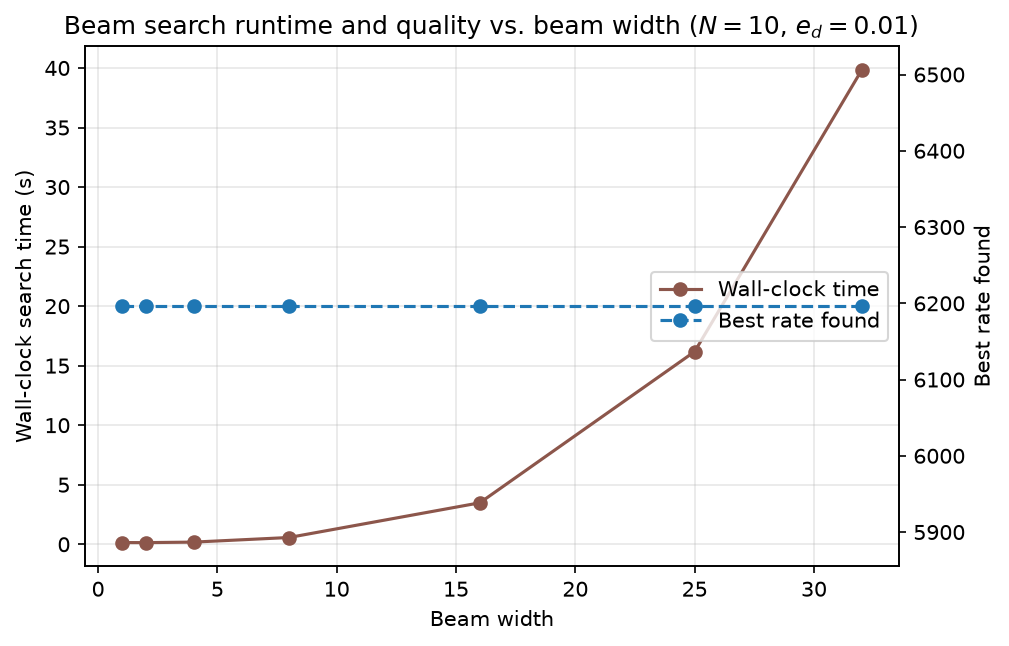
\includegraphics[width=0.75\textwidth]{figures/appendix/runtime_and_quality_vs_beam_width.png}
    \caption{Beam search wall-clock time and best rate found vs.\ beam width, at $N=10$, $e_d=0.01$.}
    \label{fig:app:beamwidth}
\end{figure}
\FloatBarrier

Figure~\ref{fig:app:runtimen} extends the runtime comparison of Table~\ref{tab:benchmarks} (Section~\ref{app:runtime}) to every tested $N$: both the exact dynamic program and the beam search scale similarly with $N$ once the same-span pumping move is enabled, with the beam search consistently the faster of the two.

\begin{figure}[H]
    \centering
    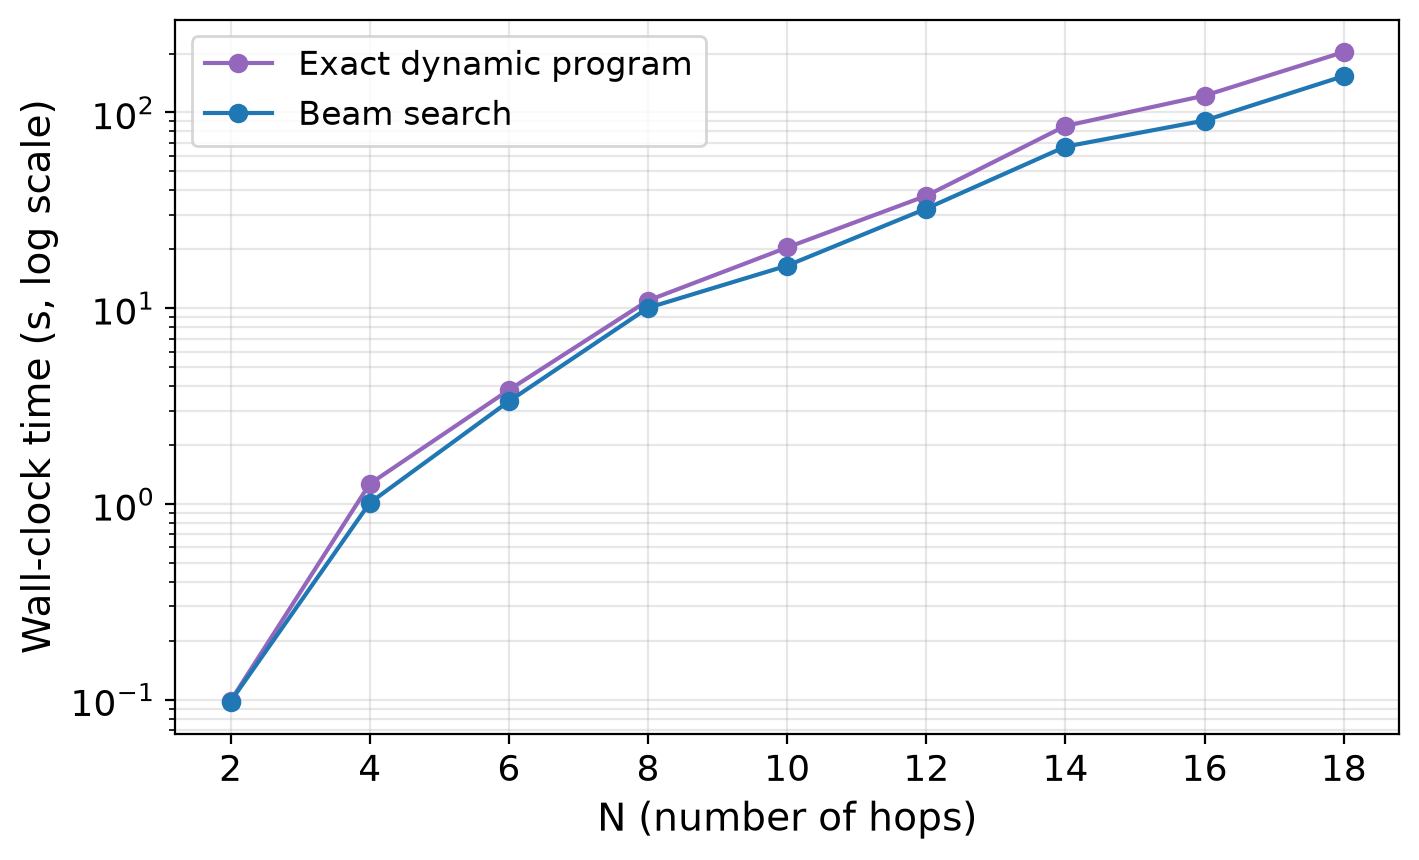
\includegraphics[width=0.75\textwidth]{figures/appendix/runtime_vs_n_pumping.png}
    \caption{Search wall-clock time vs.\ $N$ for the exact dynamic program and the beam search, same-span pumping move enabled throughout.}
    \label{fig:app:runtimen}
\end{figure}
\FloatBarrier

\subsection{Concurrent Branch Budget ($M_{\max}$)}
\label{app:mmax}

\TODO{move this subsection in appendix A below the pseudo code and make it shorter + make sure it doesn't repeat the content already discussed in that appendix A}

Section~\ref{sec:model:scope} notes that $M_{\max}$, the number of concurrently open branches (Section~\ref{sec:model:budget}), is computed exactly for a given schedule but is not used to prune the search itself. Table~\ref{tab:app:mmax} gives $M(\Sigma)$ for the fixed schedule families and the optimizer's own budget-relaxed best schedule across $N=2$ to $N=18$ at $e_d=0.01$: no family shows $M(\Sigma)$ growing with $N$, since the register-allocation bound (Section~\ref{sec:model:budget}) is governed by \Gls{dag} depth and branching shape rather than hop count. Bisecting $m_{\max}$ downward from the unconstrained optimum at $N=10$, $E_{\max}=100$ shows that the budget-relaxed optimum ($M=4$) remains selectable down to $m_{\max}=4$, but no candidate in the beam-searched frontier clears both the rate objective and $m_{\max}=3$, at which point $M_{\max}$ becomes the actual binding constraint rather than $E_{\max}$ or $F_{\min}$.

\begin{table}[h]
    \centering
    \small
    \begin{tabular}{cccc}
        \hline
        $N$ & Raw chain & Heralded end-node pumping & Optimizer (budget-relaxed) \\
        \hline
        2  & 3 & 4 & 3 \\
        4  & 3 & 4 & 4 \\
        6  & 3 & 4 & 4 \\
        8  & 3 & 4 & 4 \\
        10 & 3 & 4 & 4 \\
        14 & 3 & 4 & 4 \\
        18 & 3 & 4 & 5 \\
        \hline
    \end{tabular}

    \caption{$M(\Sigma)$ vs.\ $N$ for the fixed schedule families and the budget-relaxed optimum, $e_d=0.01$.}
    \label{tab:app:mmax}
\end{table}

\subsection{Runtime Benchmarks}
\label{app:runtime}

Table~\ref{tab:benchmarks} gives the wall-clock time and returned score underlying Figure~\ref{fig:app:runtimen} and the beam-width discussion above, at representative chain lengths, together with the two cases (footnoted in the table) where the pumping-enabled exact dynamic program is not a strict upper bound on beam search (Section~\ref{sec:alg:pumping}).

\begin{table}[ht]
    \centering
    \small
    \begin{tabular}{rrllrr}
        \toprule
        $N$ & $E_{\max}$ & Exact DP (s) & Beam search (s) & Exact DP score & Beam search score \\
        \midrule
        2  & 20  & 0.10 & 0.10 & 50\,000 & 50\,000 \\
        6  & 60  & 3.82 & 3.34 & 14\,372\textsuperscript{$\ddagger$} & 15\,391 \\
        10 & 100 & 20.43 & 16.50 & 6\,196 & 6\,196 \\
        14 & 140 & 85.37 & 66.93 & 3\,394 & 3\,394 \\
        18 & 180 & 203.68\textsuperscript{$\dagger$} & 153.52 & $-\infty$ & 1\,214 \\
        \bottomrule
    \end{tabular}

    \caption{Wall-clock runtime and returned score for the exact dynamic program and beam search at representative chain lengths. Runs use $E_{\max}=10N$, $F_{\min}=0.9$, beam width $w_{\mathrm{beam}}=25$, same-span pumping enabled (Section~\ref{sec:alg:pumping}), a 300~s timeout, and a 3~GiB memory limit. The score is the value of the active objective; here, it is the returned schedule rate $R(\Sigma)$. \textsuperscript{$\dagger$}At $N=18$, the exact dynamic program completes within the timeout but finds no feasible candidate, while beam search returns a feasible one. \textsuperscript{$\ddagger$}At $N=6$, beam search returns a higher score than the exact dynamic program. These cases arise because same-span pumping is itself beam-limited, so the pumping-enabled exact dynamic program is not guaranteed to upper-bound beam search (Section~\ref{sec:alg:pumping}).}
    \label{tab:benchmarks}
\end{table}

\section{Timing Sensitivity, Full Sweeps}
\label{app:timing}

% Source: outputs/sweep_gamma_and_tau_emit/README.md

Section~\ref{sec:exp:timing} summarizes the effect of memory dephasing and generation latency on schedule rate and fidelity; Figure~\ref{fig:timing} gives both sweeps in full, at $N=10$ and $e_d=0.01$.

\paragraph{Memory dephasing ($\gamma$)}

Sweeping $\gamma$ from 0 to $10^5$ leaves the raw chain and paper schedule's fidelity unchanged across the tested range: neither contains a resource that waits for another branch to become ready, so the simulated execution introduces no additional memory-decoherence interval for these schedules. By contrast, heralded end-node pumping falls from $F=0.92$ at $\gamma=0$ to $F=0.25$, the maximally mixed limit, at $\gamma=10^5$, because its sacrificial copies remain stored while each round-trip heralding delay is incurred. The schedules selected by the optimizer remain flat across the tested values of $\gamma$; this does not mean memory dephasing is generally harmless, only that the search favours optimistic schedules in which the relevant intermediate heralding delays are deferred, avoiding the specific waiting pattern that causes the collapse of the heralded pumping schedule (Section~\ref{sec:disc:optimistic}).

\paragraph{Generation latency ($\tau_{\mathrm{emit}}$)}

Sweeping $\tau_{\mathrm{emit}}$ at $\gamma=0$ reduces the rate monotonically for every schedule. The relative rate loss is largest for the optimistic pumping family, whose baseline latency is approximately $1\times L/c$, and smallest for heralded end-node pumping, whose baseline latency is approximately $9\times L/c$: a schedule that already has a larger fixed latency is proportionally less affected by the same additional per-photon generation delay. The two schedules cross near $\tau_{\mathrm{emit}}\approx0.01$; above this value, the larger fixed latency of heralded pumping makes it less sensitive, in relative terms, to further increases in generation latency.

\begin{figure*}[ht]
    \centering
    \begin{subfigure}[b]{0.48\textwidth}
        \centering
        
\includegraphics[width=\textwidth]{figures/results/gamma_fidelity.png}
        \caption{Fidelity vs.\ $\gamma$}
    \end{subfigure}
    \hfill
    \begin{subfigure}[b]{0.48\textwidth}
        \centering
        
\includegraphics[width=\textwidth]{figures/results/tau_emit_rate.png}
        \caption{Rate vs.\ $\tau_{\mathrm{emit}}$ (log-log)}
    \end{subfigure}
    \caption{Timing sensitivity of the raw chain, the paper schedule, and heralded end-node pumping, at $N=10$ and $e_d=0.01$.}
    \label{fig:timing}
\end{figure*}
\FloatBarrier

\section{Schedule DAGs of Selected Optima}
\label{app:dags}

The schedules found in Chapter~\ref{chap:experiments}, such as the budget-relaxed optimum at $N=10$ (Section~\ref{sec:exp:headline}), are automatically constructed \Glspl{dag} with 50 to 100 \texttt{GenNode} leaves and several hundred nodes once every backbone and purification step is counted. Rendered at a scale where individual node labels stay legible, such a diagram does not fit within a single printed page: the same rendering tooling used for the worked $N=2$ example of Figure~\ref{fig:model:dag-example} produces images several thousand pixels wide once applied to these larger, automatically-constructed schedules, since node count (not page size) is the limiting factor.

Reproducing one of these diagrams here at a reduced scale would not add information beyond what Chapter~\ref{chap:experiments}'s tables and the Pareto frontier of Figure~\ref{fig:pareto} already convey, namely each schedule's cost, fidelity, rate, and overall shape family (e.g.\ end-node pumping vs.\ a span-partition structure), while making every individual node illegible. Figure~\ref{fig:model:dag-example} therefore remains the representative illustration of the \Gls{dag} representation itself, at a size deliberately chosen to exercise every node type from Section~\ref{sec:model:dag} while staying legible; the full artifacts for every optimum discussed in this thesis are reproducible directly from the search calls and parameters documented in Chapter~\ref{chap:algorithms} and Table~\ref{tab:params}.